\documentclass[12pt,a4paper,twoside]{article}
\usepackage{polski}
\usepackage[utf8]{inputenc}
\usepackage[left=3.5cm,right=2.5cm,top=2.5cm,bottom=2.5cm]{geometry}
\usepackage{graphicx}
\usepackage{lipsum}
\usepackage{setspace}
\usepackage{xcolor}
\title{Aplikacja do zarządzania zbiorami danych}
\spacing{1.5}
\setlength{\parindent}{1.25cm}
%% ########################################################
\begin{document}
\thispagestyle{empty}
\begin{center}

\includegraphics[width=\textwidth]{img/logo_AGH.jpg}\\
{\bf{\sf WYDZIAŁ GEOLOGII, GEOFIZYKI I OCHRONY ŚRODOWISKA}}\\[5mm]
%% ======================================================
{\bf{\sf{KATEDRA GEOINFORMATYKI I INFORMATYKI STOSOWANEJ}}}\\[14mm]

{\sf{\huge Projekt dyplomowy}}\\[12mm] 
%% ======================================================
{\sf{\Large Aplikacja do zarządzania zbiorami danych\\[2mm] 
Dataset management application}}\\[40mm]
\end{center}
{\sf\begin{tabular}{ll}
	Autor: & Monika Hertel\\
	Kierunek studiów: & Inżynieria i Analiza Danych\\
	Opiekun pracy: & dr Paweł Oleksik\\
\end{tabular}}\\[10mm]
\begin{center}
{\sf Kraków, 2024}
\end{center}
%% ########################################################
\newpage
\subsection*{Abstrakt}
Celem pracy inżnierskiej jest przedstawienie projektu aplikacji wspomagającej gromadzenie i segregację plików z danymi ze względu na ich zawartość. Zostaną opisane możliwe implementacje dotyczące obsługi zbiorów danych. Praca skupia się na elementach realizacji związanej z plikami tekstowymi, a w szczególności na formacie PDF. System wykorzystuje architekturę webową lecz tworzy własny interfejs graficzny.\newline\newline
\textbf{Słowa klucze}: Przechowywanie danych, streszczenia, aplikacja natywna, analiza tekstu.
%Zgromadzone dane mogą być przechowywane w różnych formach (pliki w systemie plików, rekordy w bazach danych), jak i w różnych miejscach (lokalne nośniki danych, zasoby w chmurze). Szczególnym przypadkiem są pliki PDF, gdzie proces ekstrakcji zawartości jest utrudniony w związku z kodowaniem i formatem pliku, co zostanie omówione w dziale 1.2. Bazy danych powyższego rodzaju wyróżniają się w scenariuszach, w których elastyczność, skalowalność i wydajność są najważniejsze, znajdując zastosowanie w aplikacjach internetowych, analityce danych w czasie rzeczywistym (np. monitorowanie stanu systemu) i środowiskach zajmujących się dużymi ilościami nieustrukturyzowanych lub częściowo ustrukturyzowanych danych. Python to język programowania wysokiego poziomu znany ze swojej prostoty i czytelności, Stworzenie serwera w tym języku pozwala na korzystanie z jego rozległego ekosystemu bibliotek czy szkieletów aplikacji, w szczególności narzędzi dotyczących takich tematów jak przetwarzanie i analiza danych czy sztuczna inteligencja [14]. Zmienność w użyciu słów kluczowych, takich jak synonimy, skróty lub różnice w pisowni, może stanowić wyzwanie w dokładnej identyfikacji i wyodrębnianiu odpowiednich słów kluczowych z zawartości pliku. Dla człowieka proces identyfikacji elementów obrazu dzieje się podświadomie, a w przypadku programu, jest on w stanie rozpoznać i przypisać grafikę do odpowiedniej kategorii, jedynie w sytuacji gdy jest on zaprogramowany do wykrywania ich.
\newpage
\tableofcontents
\newpage
\section*{Wstęp}
\addcontentsline{toc}{section}{Wstęp}
Niniejsza praca ma na celu prezentacje projektu aplikacji, która umożliwiłaby użytkownikowi gromadzenie i zarządzanie zbiorami danych. Przedstawia elementy implementacji i potencjalne rozszerzenia aplikacji.\par
Aplikacja ułatwiłaby użytkownikom importowanie i przechowywanie plików zawierających informacje. Pliki te, określane zbiorczo jako zbiór danych, obejmują szeroki zakres typów treści, między innymi artykuły naukowe, dane tabelaryczne czy pliki tekstowe. System, po rozpoznaniu formatu danych, przetwarzał i analizowałby ich zawartość, aby wspomóc proces klasyfikacji. 
Został zaprojektowany jako proste rozwiązanie programowe do indywidualnego użytku z możliwością wyposażenia\break w rozszerzenia, które wykorzystują techniki sztucznej inteligencji (AI). \par
Praca zaprezentuje kluczowe komponenty aplikacji, takie jak moduł gromadzenia danych, mechanizm kategoryzacji czy wyszukiwania. Zostanią przedstawione schematy działania tych funkcjonalności. 
\newpage
%% ########################################################
\section{Zagadnienia dotyczące projektu}
%Gromadzone dane można przechowywać w różnych formach (pliki w systemie plików, rekordy w bazach danych) i w różnych miejscach  (lokalne nośniki, zasoby w chmurze). W tej wersji projektu, ze  względu na przewidywaną skalę, zdecydowano się na składowanie danych w nierealcynej bazie danych zarządzanej silnikiem MongoDB. Omówienie różnych aspektów przechowywania danych znajduje się w r.1.1
Zaprojektowany system jest przeznaczony do gromadzenia i klasyfikowania danych dla indywidualnego użytkownika. Zgromadzone dane mogą być przechowywane\break w różnych formach (pliki w systemie plików, rekordy w bazach danych), jak\break i w różnych miejscach (lokalne nośniki danych, zasoby w chmurze). Ze względu na przewidywaną skalę tej wersji projektu, zdecydowano się na składowanie danych w nierelacynej bazie danych zarządzanej silnikiem MongoDB. Omówienie różnych aspektów przechowywania danych znajduje się w rozdziale 1.1.\par
Zamysłem aplikacji jest wspomaganie klasyfikacji gromadzonych danych. Aby było to możliwe należy wydobyć informacje z pliku, a następnie odpowiednio je przetworzyć. Sposób wydobywania właściwych informacji i ich przekształcania zależy od rodzaju danych (dokumenty tekstowe, dane tabelaryczne, grafiki).
Szczególnym przypadkiem są pliki PDF, gdzie proces ekstrakcji zawartości jest utrudniony\break w związku z kodowaniem i formatem pliku, co zostanie omówione w dziale 1.2. \par
W pracy skupiono się na przedstawieniu elementów przetwarzania plików tekstowych. Dla nich zdecydowano się na wykorzystanie informacji pod kątem kreacji streszczeń zawartości, jak i generacji słów kluczowych. Etykiety służyłyby do kategoryzacji plików względem tematu. W punkcie 1.3 opisano problem tworzenia abstraktów, metody oraz sposoby sprawdzania poprawności.\par
Projekt zakłada wykorzystanie architektury webowej, która jest specyficzną realizacją architektury typu klient-serwer. Zazwyczaj klientem jest przeglądarka,\break a komunikacja z serwerem odbywa się poprzez protokół HTTP.
W realizacji, dzięki wykorzystaniu pakietu Electron, finalna aplikacja nie wymaga użycia zewnętrznej przeglądarki, dzięki czemu zachowuje się ona jak aplikacja natywna. Opis architektury webowej oraz pakietu Elektron został umieszczony w punkcie 1.4. 
%% ########################################################
\clearpage
\subsection{Sposoby przechowywania informacji}
Istnieje wiele sposobów magazynowania danych. Wybór odpowiedniego sposobu zależy od indywidualnych potrzeb użytkownika oraz ilości informacji. 
Na poziomie organizacji dzielą się one na serwery lokalne (\textit{ang. on-premise}) oraz przechowywanie w chmurze (\textit{ang. cloud storage}). Na niższym poziomie architektury, dane mogą być przechowywane z wykorzystaniem baz danych czy plików w systemie plików.\par
\subsection*{Bazy danych}
Bazy danych dzielą się na bazy SQL (\textit{ang. Structured Query Language}) oraz NoSQL (\textit{ang. Not only SQL}). Najważniejszym czynnikiem rozróżniającym te bazy jest model przechowywania danych. Bazy danych SQL charakteryzują się ustrukturyzowanym modelem danych oraz porządkują informacje w tabele z predefiniowanymi schematami. Wykorzystywane są w sytuacjach gdzie wymagane jest zagwarantowanie spójności danych oraz zastosowanie złożonych zapytań czy transakcji, jak np.\break w systemach finansowych.\par
Bazy NoSQL oferują elastyczny model przechowywania, który obsługuje różne struktury danych. Obsługują różnorodne języki zapytań lub interfejsy API dostosowane do określonych typów baz danych, zaspokajając indywidualne potrzeby w zakresie zarządzania danymi. Bazy danych powyższego rodzaju wyróżniają się w scenariuszach, w których elastyczność, skalowalność i wydajność są najważniejsze, znajdując zastosowanie w aplikacjach internetowych, analityce danych w czasie rzeczywistym (np. monitorowanie stanu systemu) i środowiskach zajmujących się dużymi ilościami nieustrukturyzowanych lub częściowo ustrukturyzowanych danych \cite{novssql}.\par
Na potrzeby projektu wykorzystano bazę typu NoSQL, a dokładniej MongoDB. Elementem stojącym za tą decyzją była niezdefiniowana struktura rekordów powstałych w wyniku działań systemu. \par
MongoDB przechowuje dane w dokumentach, które składnią przypominają JSON, umożliwiając dynamiczny schemat i łatwą integrację z systemami o architekturze klient-serwer \cite{mongodb}. 
\subsection*{Serwery lokalne a chmura}
Gdy rozmiar bazy danych przekracza dedykowany rozmiar pamięci masowej prywatnych urządzeń, takich jak komputery osobiste lub dyski zewnętrzne, lub gdy jej obecność zaczyna ograniczać funkcjonalność poszczególnych systemów komputerowych, należy rozważyć przeniesienie danych na serwer lokalny lub do infrastruktury opartej na chmurze.\par
Pojęcie \textbf{serwerów on-premises} odnosi się do fizycznego sprzętu i infrastruktury, które znajdują się pod kontrolą organizacji lub osoby fizycznej. Podejście to obejmuje konfigurowanie i utrzymywanie serwerów na miejscu w celu przechowywania danych i zarządzania nimi, bez angażowania usługodawców zewnętrznych \cite{F2023}.\par
Usługi \textbf{przechowywania w chmurze}, takie jak Amazon Web Services (AWS) czy Azure Cloud, zapewniają możliwość przechowywania danych i zarządzania nimi w zdalnych centrach danych. Możliwe jest zapewnienie redundancji zasobów poprzez przechowywanie ich w więcej niż jednym miejscu. Chroni to przed utratą danych\break w wypadku nieprzewidywalnych zdarzeń (awarie, klęski żywiołowe).\par
Wybór miejsca przechowywania danych zależy od takich czynników, jak wymagania bezpieczeństwa, potrzeby skalowalności czy ograniczenia budżetowe. Często korzystne jest przyjęcie podejścia hybrydowego lub wielochmurowego, wykorzystującego mocne strony różnych opcji przechowywania danych \cite{Ho2022}.\par
\subsection{Ekstrakcja tekstu plików PDF}
Pliki PDF są powszechnie przyjętym standardem przechowywania informacji. Format PDF jest oparty o binarną strukturę pliku, zoptymalizowanego pod kątem wysokiej wydajności odczytu wizualnego oraz wydruku. Zawierają w sobie informacje o strukturze dokumentu, takie jak zawartość tekstowa, grafiki czy użyta czcionka. Format PDF separuje informacje dotyczące samego znaku od jego wizualnej reprezentacji. Jest to rozróżnienie na znak pisarski (grafem) i glif, gdzie grafem jest jednostką tekstu a glif, jednostką graficzną. Glif informuje o położeniu znaków na stronie dokumentu, jego czcionce i innych elementach wyglądu.\par Niezaszyfrowane PDF mogą być w całości reprezentowane z użyciem znaków ze zbioru zdefiniowanego w \textit{ANSI X3.4-1986}, tj. znaków kodowanych na 7 bitach. Wizualnie jednak nie są one ograniczone do zbioru ASCII \cite{ISO32000}. W przypadku liter nie łacińskich czy znaków matematycznych, są one zapisywane w postaci 2-bitowej wartości odpowiadającej znakowi w kodowaniu \textit{Unicode} np. $<0020>$.\break Glif takiego fragmentu posiada również wartość \textit{toUnicode}, a w przypadku jej braku, informacja o znaczeniu będzie niedostępna. \par
Otrzymanie zawartości pliku może być wykonane za pomocą wydobycia elementów PDF z strumienia pliku lub z użyciem analizy obrazów, na przykład technologi optycznego rozpoznawania znaków OCR (\textit{ang. Optical Character Recogintion}). 
Podstawowym zadaniem systemu OCR jest konwersja dokumentów w dane możliwe do edytowania czy wyszukiwania. Techniki oparte o analizę obrazów są bezpośrednio zależne od jakości wprowadzonego elementu. Idealną sytuacją dla wykorzystania metod OCR jest kiedy posiadany plik zawiera w sobie jedynie tekst i jest obrazem binarnym \cite{mithe2013optical}. Dodatkowym atutem takich systemów jest możliwość wykrycia pisma i jego konwersja na tekst.\par
Ekstrahowanie danych ze strumienia pliku, wiąże się z kilkoma problemami. Biorąc pod uwagę, że plik PDF może posiadać różne schematy kodowania takie jak \textit{UTF-8}, \textit{ASCII} czy \textit{Unicode}, możemy doświadczyć utraty informacji. Automatyczna ekstrakcja zawartości polega na selekcji znaków znajdujących się pomiędzy zdefiniowanymi słowami kluczowymi. Pliki PDF są przystosowane do drukowania, z tego powodu reprezentacja tekstu w strumieniu może się znacząco różnić od tej na stronie. Ponieważ pozycje znaków na poszczególnych stronach są absolutne, przedstawienie w strumieniu bierze pod uwagę koordynaty elementów.\par
Niezależne od sposobu pobierania informacji, nie jest możliwe zagwarantowanie ich poprawności względem dokumentu wejściowego. Brak formalnej definicji struktury, przynajmniej jeżeli chodzi o artykuły naukowe, uniemożliwia stworzenie uniwersalnego algorytmu ekstrakcji.
%%#########################################
\subsection{Problem tworzenia streszczeń}
Streszczenie artykułu naukowego jest jego kluczowym elementem. Ilość informacji dostępnych dla każdego, kto szuka wiedzy na dany temat, może być przytłaczająca. Jego celem jest przekazanie najważniejszych elementów treści, aby czytelnik mógł określić, czy informacje są dla niego istotne. \par
W kontekście uczenia maszynowego, kondensacja treści w celu stworzenia abstraktu, najczęściej opiera się na obliczaniu poziomu istotności dla każdego zdania \cite{MUTLU2020102359}. Skracając czas potrzebny na napisanie abstraktu, automatyzacja ma na celu ułatwienie autorom pisania artykułów. Systemy ATS (ang. \textit{Automatic Text Summarization}) są jednym z cięższych wyzwań sztucznej inteligencji, dotyczących przetwarzania języka naturalnego \cite{ELKASSAS2021113679}. Podejścia do tworzenia tych systemów, możemy podzielić na ekstraktywane, abstrakcyjne i hybrydowe. 
\subsubsection{Metody ekstraktywne a abstrakcyjne}
Większość badań nad systemami ATS skupia się na użyciu metod ekstraktywnych, starając się przy tym uzyskać zwięzłe i kompletne streszczenia. Podejście ekstraktywne polega na wybraniu najważniejszych zdań z całego dokumentu, a długość uzyskanego wyniku zależy od wartości stopnia kompresji \cite{Gambhir2017}. \par
Streszczenia stworzone z użyciem metod abstrakcyjnych wymagają głębszej analizy tekstu wejściowego. Generują one podsumowanie poprzez "zrozumienie" głównych pojęć w dokumencie wejściowym. Dzieje się to poprzez implementacje złożonych algorytmów przetwarzania języka naturalnego (\textit{ang. NLP, Natural Language Processing}). Następnie dokonywane jest parafrazowanie tekstu w celu wyrażenia tych pojęć z użyciem słów, które nie należą do oryginalnego tekstu. W praktyce rozwój wspomnianych systemów wymaga kompleksowych zbiorów danych.\par
Istnieje również podział technik tworzenia streszczeń na nienadzorowane\break i nadzorowanie. Nienadzorowane tworzą streszczenia tylko na podstawie danych wejściowych, czyli jedynie zawartości wprowadzanego dokumentu. Próbują one odkryć ukrytą strukturę w nieoznakowanych danych. Techniki te są zatem odpowiednie dla wszelkich nowo zaobserwowanych danych nie wymagających modyfikacji.\par
Sposób nadzorowany wymaga trenowania modelu, jak i wprowadzenia opisanego zbioru treningowego. Takie zbiory powinny posiadać docelowe postacie streszczeń otrzymane z pełnego tekstu dokumentu. Taki proces jest trudny do przeprowadzenia na większej ilości tekstów \cite{ELKASSAS2021113679}.
\subsubsection{Ocena poprawności abstraktu}
Zazwyczaj ingerencja człowieka jest wymagana przy ewaluacji wytworzonego streszczenia. Treść jest sprawdzana pod kątem poprawności gramatycznej, składni czy całościowej spójności. Taka ewaluacja wymaga dużego nakładu pracy, a przy większych projektach jest praktycznie niemożliwe. Dlatego automatyzacja tego procesu jest wręcz wymagana.\par
Jednymi z pierwszych metod ewaluacji automatycznej były metryki takie jak podobieństwo cosinusowe (\textit{ang. cosine similarity}), \textit{unit overlap} czy miara najdłuższego wspólnego podzdania (\textit{ang. longest common subsequence}). Te elementy zostały później skondensowane w zbiór kryteriów opisanych akronimem \textit{ROUGE} (\textit{ang. Recall-Oriented Understudy of Gisting Evaluation}) \cite{rouge}. Poniższy segment przedstawia poszczególne komponenty zestawu \textit{ROUGE}, to jest kryteria \textit{ROUGE-N}, \textit{ROUGE-L} oraz \textit{ROUGE-S}.\par
\begin{itemize}
	\item \textit{ROUGE-N} mierzy poziom pokrycia n-gramów, czyli ciągłych sekwencji\break \textit{n} słów, pomiędzy wytworzonym tekstem a tekstem źródłowym. Najczęstszym przypadkiem użycia tego kryterium jest ewaluacja poprawności gramatycznej. Miary \textit{ROUGE-1} oraz \textit{ROUGE-2} należą do miar \textit{ROUGE-N} i w kolejności korzystają z unigramów i bigramów.
	\item \textit{ROUGE-L} jest wyznaczana na podstawie porównania najdłuższych wspólnych sekwencji słów w zdaniach, występujących w streszczeniu wygenerowanym\break i wzorcowym. 
	\item \textit{ROUGE-S} działa na tej samej zasadzie co \textit{ROUGE-2} lecz uwzględnia w swoim działaniu struktury skip-bigram, który jest rozszerzeniem definicji bigramów o możliwość zawierania w sobie maksymalnie jednego przedimka.
\end{itemize}
\subsection{Architektura klient-server}
Architektura klient-serwer to model projektowania systemów rozproszonych, w którym zadania lub procesy obliczeniowe są podzielone między klientów i serwery.\break W tej architekturze klientami są zazwyczaj urządzenia użytkowników końcowych (takie jak komputery, smartfony lub tablety), które żądają usług lub zasobów, podczas gdy serwery są scentralizowanymi systemami, które je zapewniają \cite{client}. Architektura webowa, jako typ struktury klient-serwer, jest najczęściej wykorzystywana\break w wytwarzaniu oprogramowania internetowego z użyciem takich narzędzi jak języki opisowe HTML i CSS, czy języka Javascript. Takie aplikacje działają w przeglądarkach internetowych, lecz dzięki takim szkieletom aplikacji jak Electron, istnieje możliwość konwersji na program z własnym interfejsem graficznym, oddzielonym\break od przeglądarki. Opis tego projektu znajduje się w dalszej części rozdziału.\par
Transfer informacji między elementami aplikacji może odbywa się z pomocą protokołu komunikacyjnego jak HTTP/HTTPS (\textit{ang. Hypertext transfer protocol}). Jest to bezstanowy protokół, co oznacza, że każde zapytanie jest przetwarzane niezależne od poprzedniego. Jest on zgodny z modelem zapytanie-odpowiedź (\textit{ang. request-response}), gdzie klient wysyła proźbę a serwer odpowiada. Odpowiedź zawiera w sobie kod statusu, wymagane zasoby lub treść błędu.\par
\subsubsection{Pakiet Electron}
Electron jest oparty na Chromium, projekcie stojącym za przeglądarką Google Chrome. Oznacza to, że aplikacje wykorzystują ten sam silnik renderujący i obsługę standardów internetowych, co Chrome. Electron osadza instancję Chromium do renderowania treści internetowych w oknach aplikacji \cite{electron}.\par
Standard tworzenia aplikacji z pomocą tej biblioteki jest oparty o komunikację międzyprocesową (\textit{ang. IPC, Inter-process communication}), która jest wynikiem implementacji izolacji wątku. 
\subsubsection*{Izolacja wątku}
Separacja wątków odnosi się do możliwości izolacji różnych części aplikacji w celu zapobiegania interferencji oraz zapewnienia stabilności aplikacji. Separacja ta jest osiągana poprzez wykorzystanie wielu procesów, w tym procesu głównego i procesów renderujących.
\begin{itemize}
	\item Proces główny: zarządza cyklem życia aplikacji i interakcjami z systemem operacyjnym. Działa we własnym, odizolowanym wątku, oddzielnie od procesów renderujących.
	\item Procesy renderujące: obsługują renderowanie i wyświetlanie treści internetowych w poszczególnych oknach aplikacji. Każdy proces renderujący działa niezależnie, odizolowany od innych procesów renderujących i procesu głównego.
\end{itemize}
Separacja wątku zapewnia, że zmiany dokonane w jednej części aplikacji nie wpływają na inne części, zwiększając stabilność i bezpieczeństwo. Izolacja umożliwia również efektywne zarządzanie zasobami i skalowalność, ponieważ każdy proces może być zarządzany i optymalizowany niezależnie.
\subsubsection*{Komunikacja międzyprocesowa (IPC)}
Pomimo separacji między procesami, Electron zapewnia mechanizmy komunikacji między nimi poprzez IPC (\textit{ang. Inter-Process Communication}). Pozwala to różnym częściom aplikacji na efektywną wymianę danych, wyzwalanie akcji i synchronizację stanu.
\begin{itemize}
	\item IPC Main: Electron zapewnia moduł \textit{ipcMain} w głównym procesie, pozwalając mu nasłuchiwać i obsługiwać zdarzenia IPC wysyłane z procesów renderujących.
	\item IPC Renderer: W procesach renderujących, moduł \textit{ipcRenderer}	 umożliwia wysyłanie zdarzeń IPC do głównego procesu i odbieranie odpowiedzi.
\end{itemize}
Dzięki IPC możliwa jest implementacja dwukierunkowej komunikacji między procesem głównym a procesami renderującymi, umożliwiając im koordynację działań, udostępnianie danych i synchronizację stanu w różnych częściach aplikacji.\par
\newpage
\section{Projekt}
Celem pracy było zaprojektowanie i wykonanie programu użytkowego wspomagającego gromadzenie informacji oraz późniejsze przeszukiwanie utworzonych kolekcji. 
Wśród jego planowanych funkcjonalności należy wymienić:
\begin{itemize}
	\item możliwość gromadzenia danych różnych rodzajów (dokumenty tekstowe i hipertekstowe, dane tabelaryczne, grafiki i inne),
	\item automatyczną organizację i kategoryzację plików ze względu na zawartość,
	\item automatyczne generowanie abstraktów z dokumentów tekstowych tak, by zapewnić użytkownikowi szybki wgląd w treść bez konieczności zapoznania się\break z całą zawartością.
\end{itemize}
Docelowym odbiorcą produktu ma być indywidualny użytkownik, korzystający\break z lokalnych zasobów. Dlatego założeniem projektowym było, aby unikać używania usług zewnętrznych, np. chmurowych.
\subsection{Opis projektu}
Ze względu na rozbudowany charakter narzędzia, zostało ono zaprojektowane jako system współpracujących elementów. Są to:
%Celem systemu jest zapewnienie scentralizowanej platformy, która ułatwia efektywne gromadzenie, organizowanie i wyszukiwanie treści cyfrowych. Aplikacja ma na celu usprawnienie procesu zarządzania informacjami poprzez oferowanie takich funkcji jak:
\begin{itemize}
	\item moduł przetwarzania plików - najważniejszy moduł, decydujący jakie akcje zostaną podjęte dla danego pliku,
	\item moduł organizacji danych - segreguje dokumenty oraz tworzy połączenia między podobnymi plikami,
	\item wyszukiwarka - pobiera informacje z systemu związane z frazą wejściową\break i przedstawia użytkownikowi,
	\item moduł podsumowujący - niezależnie od rodzaju pliku tworzy skrótowy opis zawartości.
%	\item Umożliwienie użytkownikom łatwego wprowadzania do aplikacji różnych typów plików, w tym dokumentów, danych tabelarycznych, notatek i innych.
%	\item Automatyczna organizacja i kategoryzacja zebranych danych w oparciu o predefiniowane kryteria takie jak słowa klucze.
%	\item Zapewnienie użytkownikom szybkiego wyszukiwania określonych dokumentów z przechowywanych informacji za pomocą słów kluczowych, nazw plików lub innych parametrów.
%	\item Automatyczne generowanie streszczeń artykułów w celu zapewnienia użytkownikom szybkiego wglądu w treść bez konieczności czytania całego tekstu.
\end{itemize}\par
\begin{figure}[h!]
\centering
  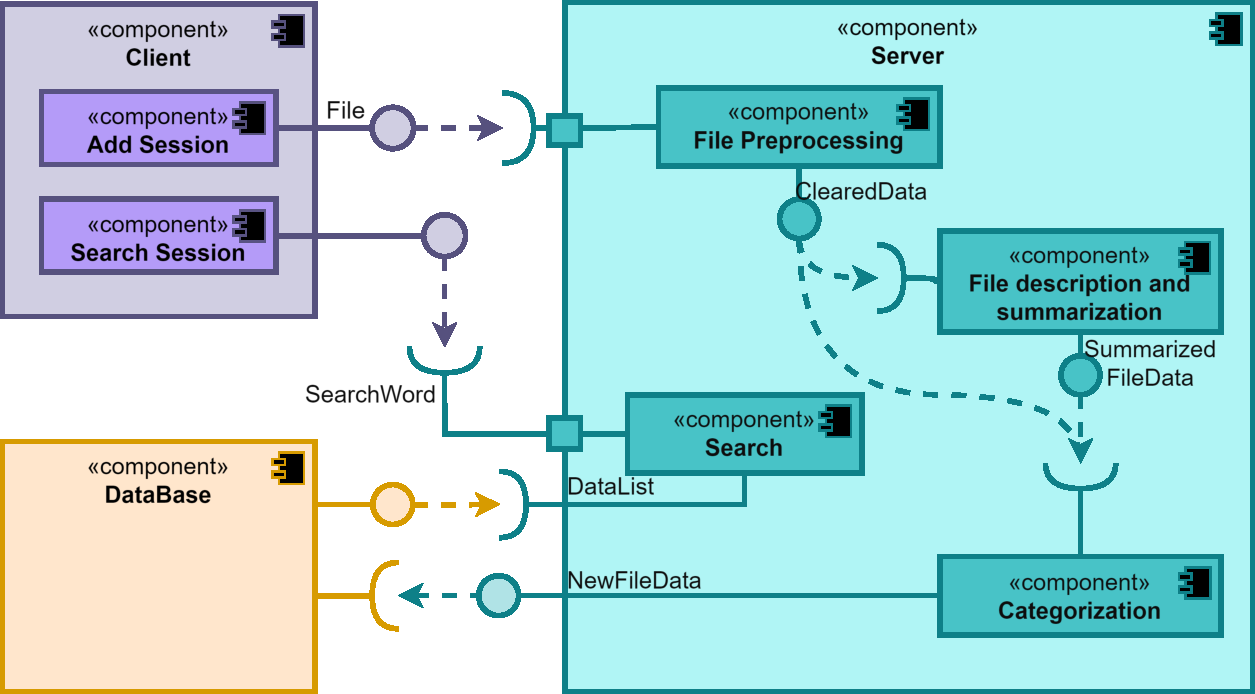
\includegraphics[width=\textwidth]{img/component.pdf}
  \caption{Diagram komponentów projektu.}
\end{figure}
%Aplikację można podzielić na kilka głównych komponentów, z których każdy pełni odrębną funkcję w systemie. Do nich zaliczamy przetwarzanie, wyszukiwanie, streszczenia, organizacja i dodawanie plików. Poniższy segment przedstawi poszczególne moduły i ich planowane możliwości.\par
\subsection{Wymagania funkcjonalne modułów}
\textbf{Moduł organizacji danych} automatycznie kategoryzuje i organizuje dane użytkownika, aby ułatwić ich efektywne wyszukiwanie i zarządzanie.
\begin{itemize}
	\item System tagowania: użytkownicy mogą samodzielnie przypisywać etykiety do każdego dokumentu lub pozostawić te wygenerowane przez system, umożliwiając im kategoryzowanie i łączenie plików w oparciu o wspólne motywy lub tematy.
	\item Struktura folderów: aplikacja zapewnia hierarchiczną strukturę folderów, która pozwala użytkownikom organizować swoje dane w zagnieżdżone kategorie, zapewniając uporządkowany i intuicyjny sposób poruszania się po zebranych informacjach.
	\item Automatyzacja: wykorzystując zaawansowane algorytmy, aplikacja analizuje zawartość elementów, aby automatycznie kategoryzować je w oparciu o cechy, takie jak słowa kluczowe, tematy lub podobieństwo treści.
\end{itemize}\par
\textbf{Wyszukiwarka} umożliwia użytkownikom szybkie i skuteczne znajdowanie określonych informacji w systemie danych.
\begin{itemize}
	\item Funkcja wyszukiwania pełnotekstowego: użytkownicy mogą przeszukiwać wszystkie elementy danych w aplikacji za pomocą słów kluczowych lub fraz, pobierając odpowiednie wyniki na podstawie pasujących treści.
	\item Zaawansowane filtry: aplikacja oferuje szereg filtrów wyszukiwania, takich jak zakres dat, typ pliku lub tag, umożliwiając użytkownikom zawężenie wyników wyszukiwania i znalezienie dokładnie tego, czego szukają.
	\item Sugestie i autouzupełnianie: gdy użytkownicy wpisują swoje zapytania, aplikacja zapewnia sugestie i opcje autouzupełniania, aby przyspieszyć proces wyszukiwania i poprawić dokładność.
\end{itemize}\par
\textbf{Moduł podsumowujący} generuje zwięzłe streszczenia dokumentów, zapewniając użytkownikom szybki wgląd w główne punkty artykułów. Realizuje też opisywanie innych rodzajów plików.
\begin{itemize}
	\item Algorytmy podsumowujące tekst: aplikacja wykorzystuje zaawansowane algorytmy do podsumowywania tekstu, które mogą obejmować metody ekstrakcyjne, które wybierają ważne zdania lub metody abstrakcyjne, które generują nową treść podsumowania.
	\item Automatyczne podsumowanie: użytkownicy mogą wybrać opcje dla automatycznego generowania podsumowań dla dokumentów w aplikacji, takie jak ilość zdań lub poziom szczegółowości podsumowań.
\end{itemize}\par
\textbf{Przetwarzanie plików} wykrywa rodzaj pliku dodanego przez klienta i wyznacza akcje do przeprowadzenia zgodnie z typem.
\newpage
\subsection{Przykładowe schematy funkcjonalności}
\subsubsection*{Dodawanie plików PDF}
Zachowanie systemu przy dodaniu plików tekstowych.
\begin{enumerate}
	\item Gdy użytkownik wybierze plik, aplikacja przesyła ścieżkę pliku do serwera.
	\item System ekstraktuje z pliku całą zawartość.
	\item Z tekstu wytwarzane są słowa klucze.
	\item W tym samym czasie jest tworzone streszczenie z użyciem algorytmu \textit{TextRank}.
	\item Jeżeli plik PDF posiada zakładki (ang. \textit{outlines}) to możemy otrzymać tytuł dokumentu i nadać plikowi taką nazwę. W przypadku ich braku tytułem pliku zostaje bazowa nazwa pliku.
	\item Ostatecznie wszystkie informacje są zbierane i przesyłane do bazy danych.
\end{enumerate}
Model TextRank zastosowany w projekcie, jest algorytmem rankingowym opartym na grafach \cite{textrank}. Operuje on na zasadach ``głosowania'' i ``rekomendacji''. Jest on używany do tworzenia streszczeń metodą ekstraktywną i nienadzorowaną. Dla przedstawionego systemu, nie jest możliwe wytworzenie odpowiedniego zbioru treningowego, aby móc zastosować metody nadzorowane. \par
Poniższy diagram przedstawia proces dodawania pliku PDF wraz z uwzględnieniem implementacji asocjacji plików o podobnej tematyce, opisanej w punkcie 2.4.3.
\begin{figure}[h!]
\centering
  \includegraphics[width=\textwidth]{img/activity\_file\_add.pdf}
  \caption{Diagram aktywności przesyłania pliku PDF.}
\end{figure}
\clearpage
\newpage
\subsubsection*{Wyszukiwanie i wyświetlanie plików}
Użytkownik ma możliwość wysukiwania plików po słowach kluczach lub tytule pliku. Tutaj przydatne jest użycie API generującego synonimy dla wyszukiwanego słowa. System zachowuje się w poniżej opisany sposób.
\begin{enumerate}
	\item Aplikacja przesyła komunikat z wyszukiwanym słowem.
	\item Serwer używając API synonimów pobiera 5 najbliższych słów do słowa szukanego.
	\item Serwer przesyła osobne komunikaty do tabeli w bazie danych, zawierające osobno słowo klucz oraz synonimy.
	\item Baza zwraca informacje dotyczące znalezionych dokumentów oraz słowo klucz.
	\item Serwer wysyła użytkownikowi posortowaną listę plików.
\end{enumerate}
\begin{figure}[h!]
\centering
  \includegraphics[width=0.8\textwidth]{img/file\_search.pdf}
  \caption{Schemat sekwencyjny wyszukiwania pliku.}
\end{figure}
%\begin{figure}[h!]
%\centering
%  \includegraphics[width=\textwidth]{img/file\_search\_code.jpg}
%  \caption{Implementacja wyszukiwania pliku}
%\end{figure}
%\newpage
\subsubsection*{Obsługa plików zawierających dane tabelaryczne}
\begin{enumerate}
	\item Użytkownik przy dodaniu pliku podaje następujące informacje.
	\begin{itemize}
		\item Czy plik zawiera informacje o nazwach kolumn, jeżeli nie to czy chce on nadać te nazwy.
		\item Czy słowa kluczowe będą nadane manualnie lub czy powinny być pobrane z nazw kolumn.
	\end{itemize}
	\item Dane są odpowiednio wczytywane na serwer do postaci ramki danych.
	\item Sprawdzany i zapisywany jest typ wartości w każdej kolumnie oraz obliczony procent ilości wartości brakujących.
	\item Dodanie rekordu do bazy danych.
\end{enumerate}
\begin{figure}[h!]
\centering
  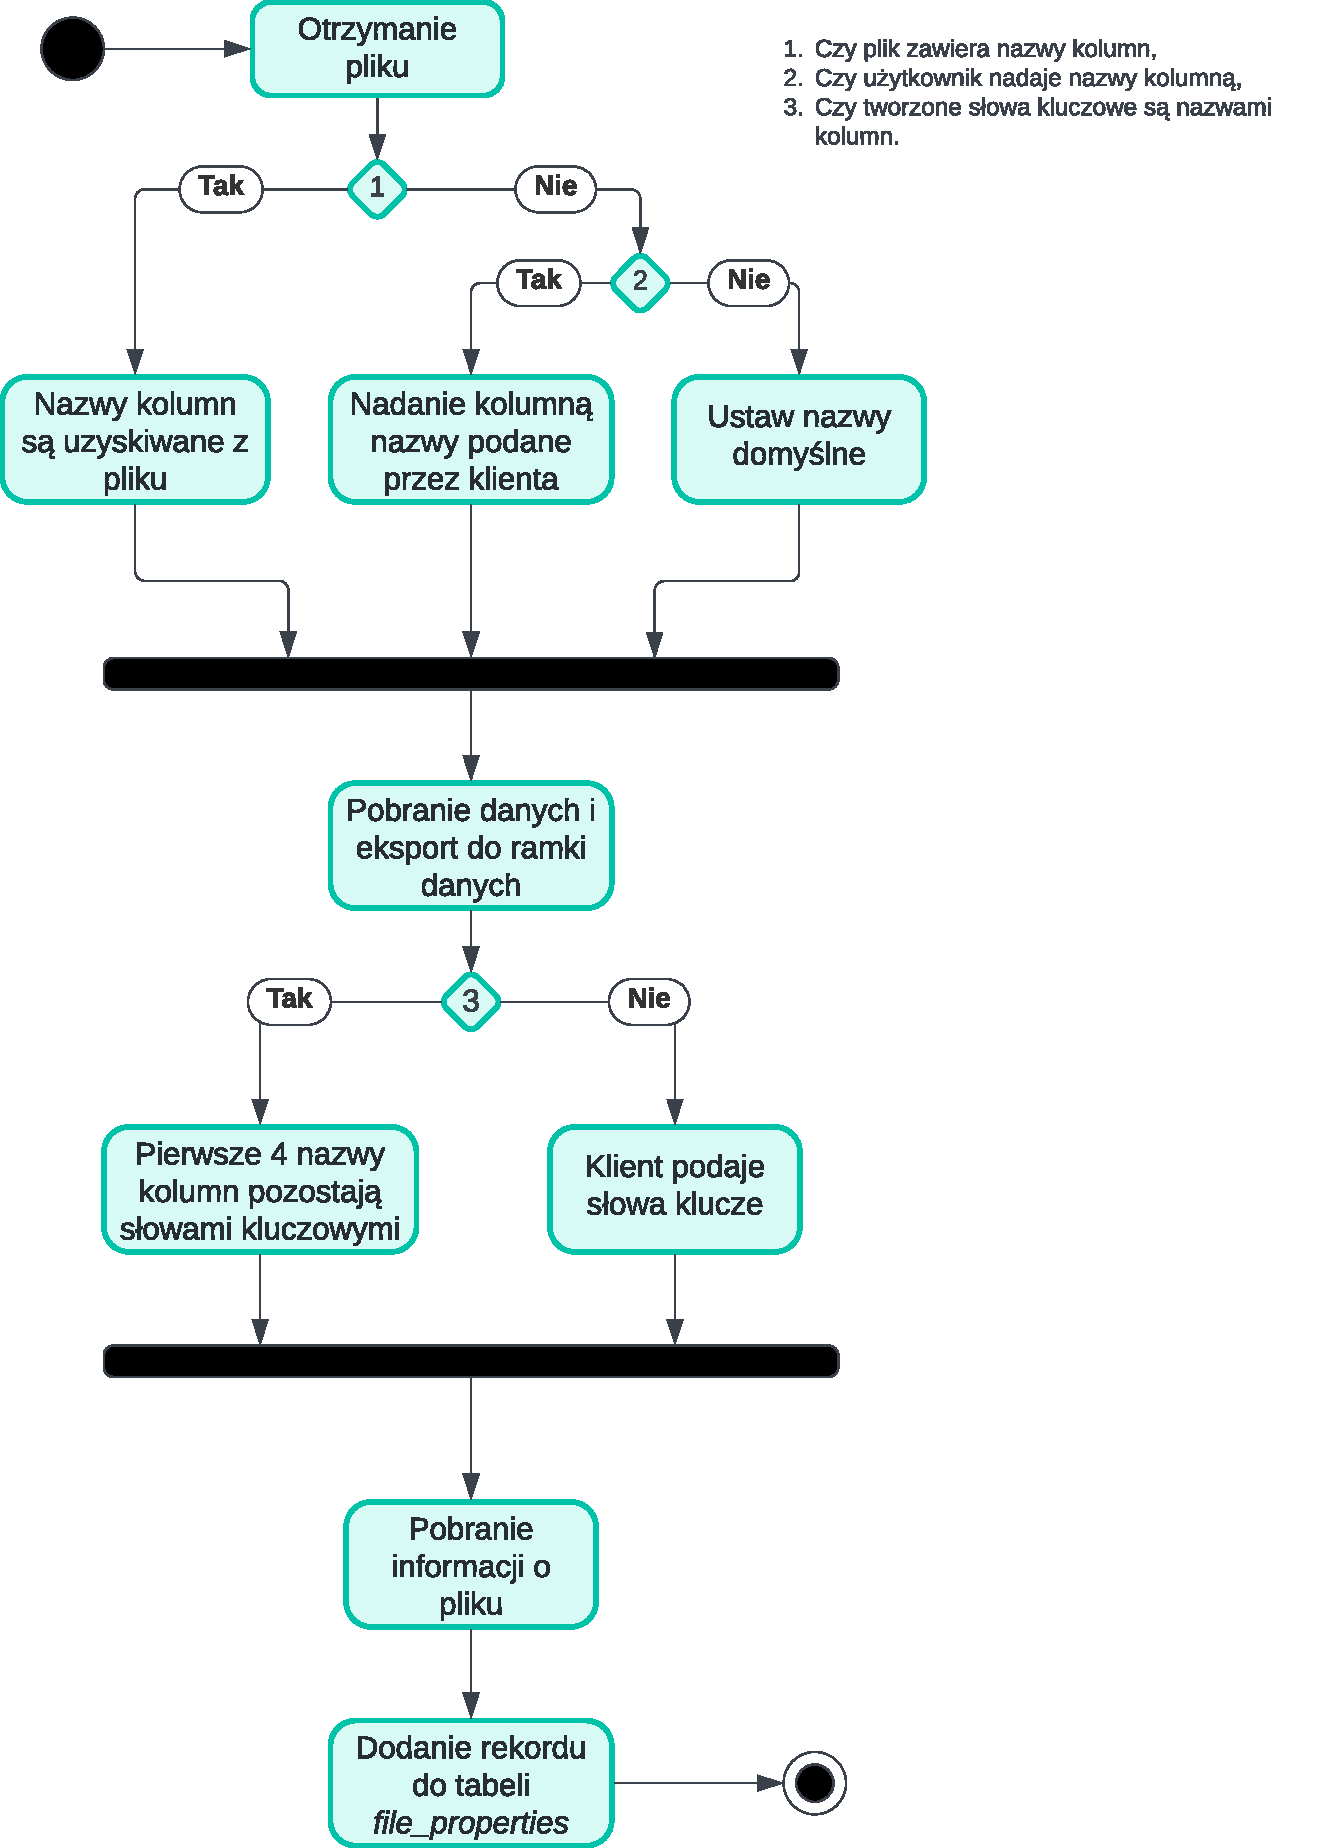
\includegraphics[width=0.9\textwidth]{img/csvac.pdf}
  \caption{Diagram aktywności przetwarzania plików tabelarycznych.}
\end{figure}
%% ########################################################
\clearpage
\newpage
\subsubsection*{Asocjacja plików o podobnej tematyce}
Poniższa sekcja przedstawia proces łączenia dokumentów na podstawie wygenerowanych słów kluczowych. System, z każdym dodanym plikiem, przeszukuje przestrzeń dokumentów i aktualizuje już utworzone rekordy, w sytuacji dopasowania. Schemat przedstawia tworzenie połączeń dla nowo dodanego pliku.
\begin{enumerate}
\item Dla każdego słowa kluczowego, jest pobrana lista ID plików z tabeli zawierającej informacje o zawartości plików, pod warunkiem dopasowania przynajmniej jednego tagu.
\item Następnie obliczany jest współczynnik podobieństwa, którego schemat postępowania jest przedstawiony poniżej.
	\begin{enumerate}
		\item Wyznaczana jest wartość dla poszczególnych słów kluczy.
		\begin{itemize}
			\item Jeżeli wysłane słowo kluczowe zgadza się fragmentarycznie z otrzymanym tagiem (np. ``zaburzenia'' a ``zaburzenia snu''), to zapisywana jest wartość $\frac{ilosc(dopasowan)}{ilosc\_slow(wejscie)+ilosc\_slow(pobrane)}$.
			\item Jeżeli słowa są identyczne, zapisywana jest wartość 1.
		\end{itemize}
		\item Wartości dla wszystkich słów kluczy są sumowane i dzielone przez liczbę tagów.
	\end{enumerate}
\item Do ID pliku przypisana jest wartość podobieństwa, i po posortowaniu od największej wartości, ID są dodawane do jednego rekordu w tabeli informującej o podobieństwach dokumentów.
	\begin{itemize}
		\item Jeżeli wartość podobieństwa nie przekracza 0.5, to plik nie jest brany pod uwagę.
	\end{itemize}
\end{enumerate}
\newpage
\section{Implementacja}
Realizacja miała na celu wykazanie możliwości projektu biorąc pod uwagę następujące aspekty. 
Po pierwsze, wykonalność aplikacji została oceniona w celu określenia jej praktyczności i potencjału pomyślnego rozwoju.
Dodatkowo przeprowadzono analizę złożoności i wymagań dotyczących zasobów związanych z przetwarzaniem różnych typów plików, skupiając się na plikach tekstowych.\par
Co więcej, wysiłki ukierunkowano na identyfikację wymaganych rozszerzeń lub ulepszeń niezbędnych do optymalizacji funkcjonalności aplikacji, ze szczególnym uwzględnieniem algorytmów klasyfikacji czy modułu tworzenia abstraktów, opartych na sztucznej inteligencji.
Wreszcie, podjęto planowanie w celu określenia zakresu wdrożenia w przydzielonych ramach czasowych, zapewniając zgodność z celami projektu i wykonalność w ramach ograniczeń dostępnych zasobów.\par
Do implementacji aplikacji użyto kombinacji technik typowych dla tworzenia aplikacji internetowych jakie zostały określone w rozdziale 1.4. Interfejs użytkownika (UI) został stworzony przy użyciu języka JavaScript, w szczególności wykorzystując bibliotekę React, wraz z językami opisu HTML i CSS do zdefiniowania struktury\break i stylizacji witryny. Jednak zamiast polegać na tradycyjnej przeglądarce internetowej, cały interfejs użytkownika został zamknięty w aplikacji natywej, dzięki wykorzystaniu szkieletu aplikacji Electron. Opis tego procesu jest zamieszczony w rozdziale 1.4.\par
Do przechowywania wyodrębnionych danych wybrano nierelacyjną bazę danych, a jako system zarządzania bazą danych wybrano MongoDB. Decyzja ta była podyktowana zróżnicowanym i niejednolitym charakterem danych, gdzie na strukturę każdego rekordu wpływają takie czynniki jak typ pliku.\par
Aby ustanowić komunikację między aplikacją a bazą danych, zaimplementowano serwer WWW przy użyciu biblioteki Flask języka Python. Działając jako istotny łącznik, serwer ten zarządza wszystkimi podstawowymi funkcjami aplikacji. Nadzoruje on zadania takie jak przetwarzanie plików, ekstrakcja danych, klasyfikacja i segregacja, wraz z wszelkimi niezbędnymi operacjami manipulacji danymi. Takie podejście zapewnia płynną interakcję między komponentami aplikacji, umożliwiając wydajną obsługę i zarządzanie danymi w całym systemie.\par
\begin{figure}[h!]
\centering
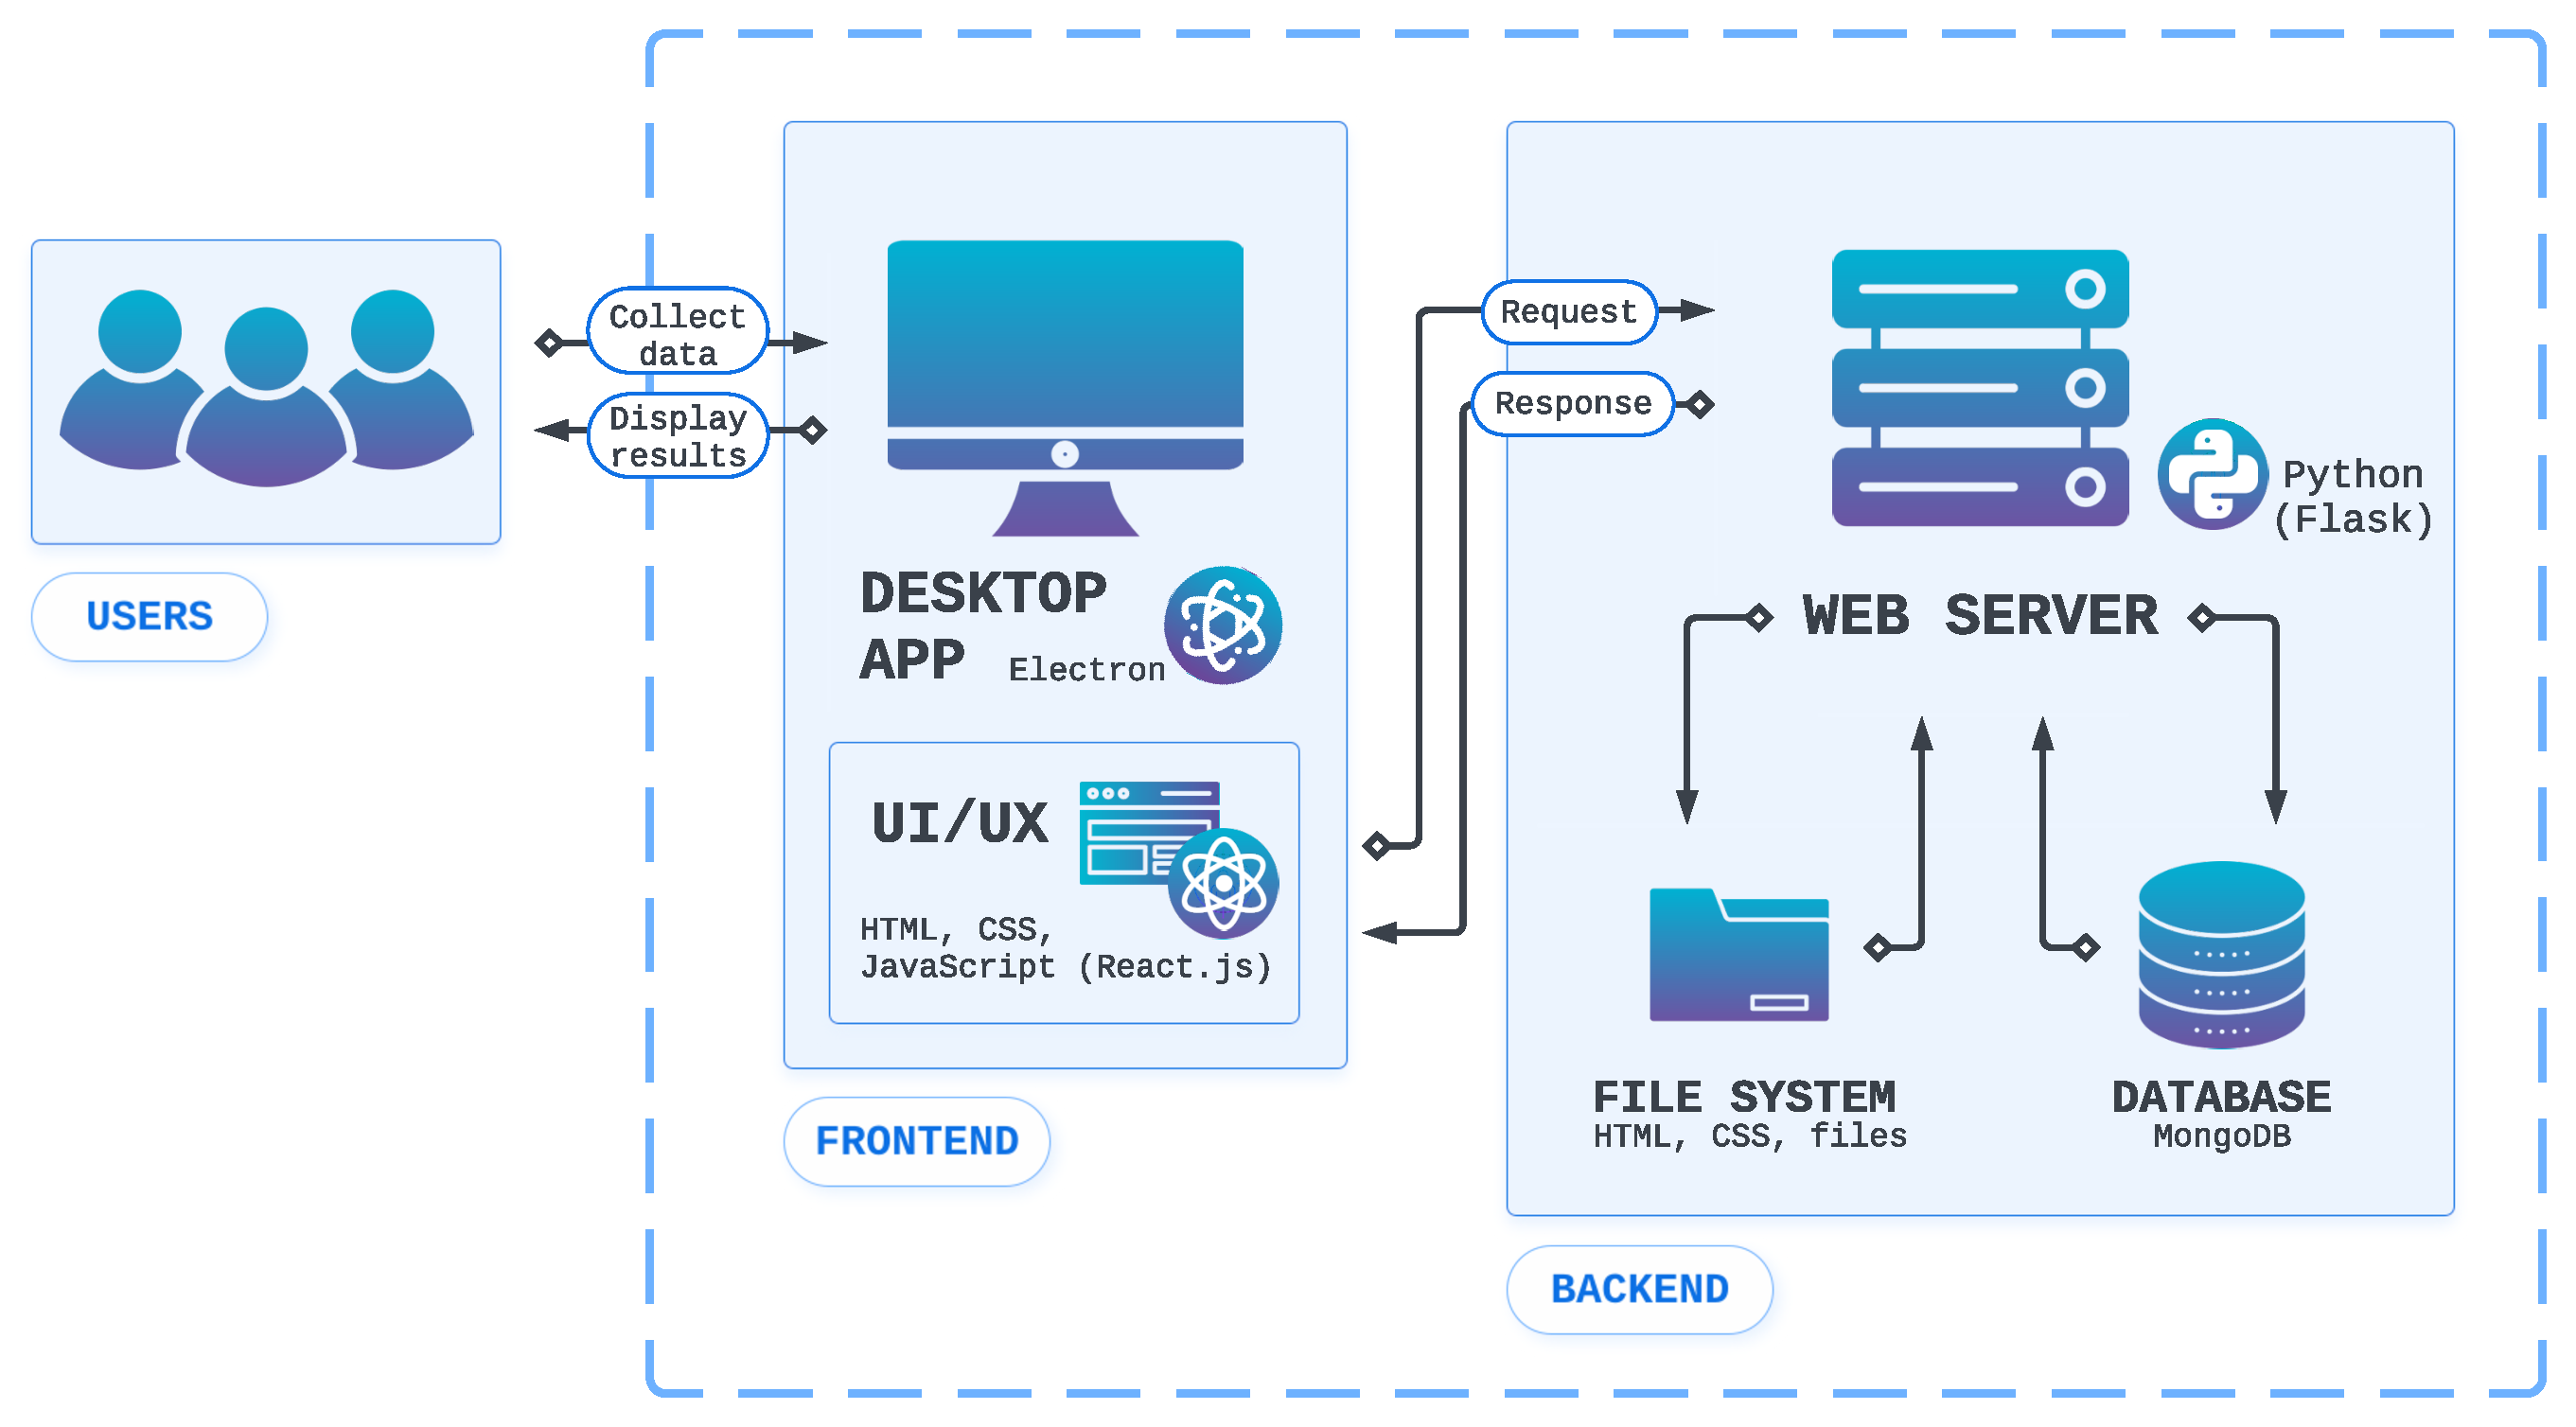
\includegraphics[width=\textwidth]{img/archi2.pdf}
\caption{Diagram struktury aplikacji.}
\end{figure}\par
\subsection{Opis wykorzystywanych elementów}
Javascript to powszechnie używany język programowania do tworzenia stron internetowych, znany ze swojej wszechstronności i kompatybilności z przeglądarkami \cite{javascript}. Opisywany system wykorzystuje Javascript w środowisku \textit{Node.js}, co ułatwia dostęp do różnorodnych pakietów takich jak \textit{React}, których opis jest przedstawiony poniżej.
\begin{itemize}
	\item \textit{React} - biblioteka pozwalająca na budowanie interaktywnych interfejsów użytkownika. Główną koncepcją React są komponenty, czyli samodzielne, hermetyczne jednostku interfejsu \cite{reactjs}.
	\item \textit{Axios} - klient HTTP z pomocą którego odbywa się komunikacja z serwerem. Jest to mechanizm oparty o obietnice (\textit{ang. promises}) pozwala na asynchroniczną relacje z punktem końcowym (\textit{ang. endpoint}). W systemie, po otrzymaniu odpowiedzi od serwera, ustawiany jest stan, czego przykład wykorzystania jest przedstawiony poniżej.
\begin{figure}[h!]
\centering
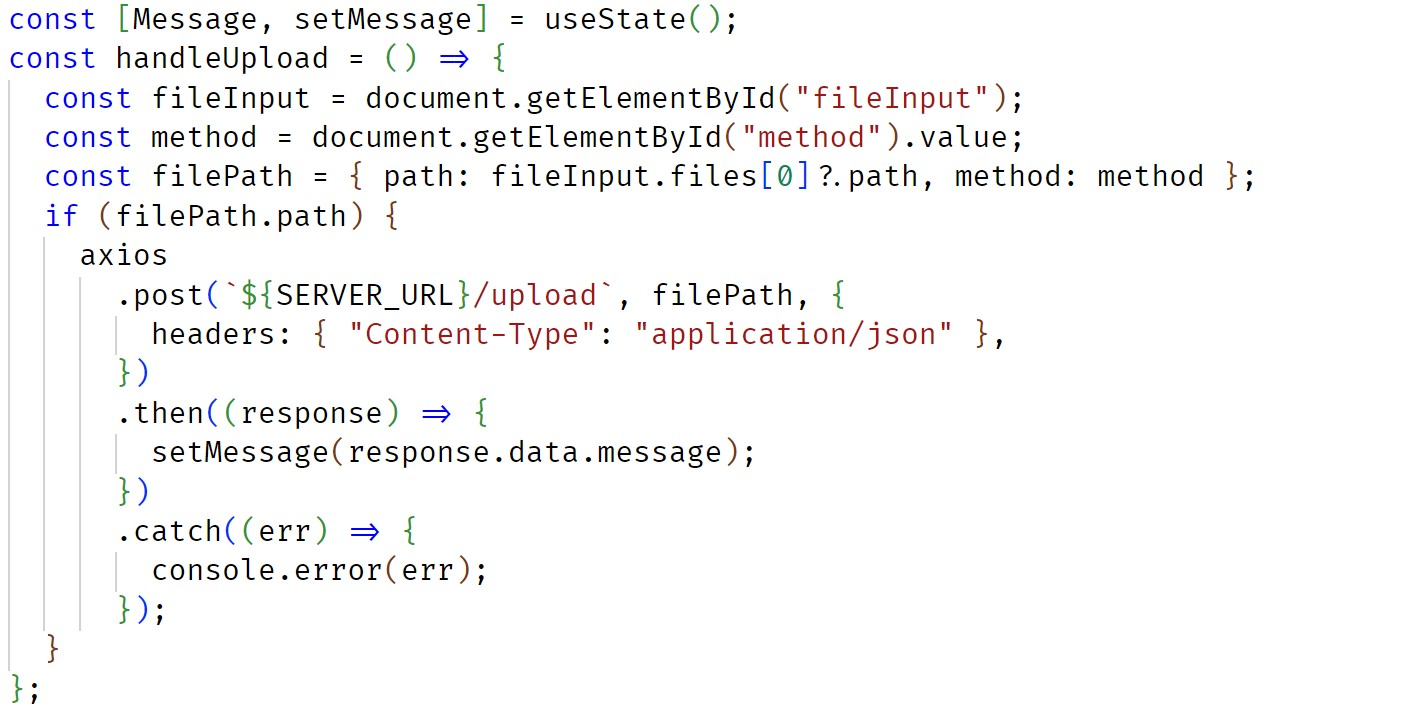
\includegraphics[width=\textwidth]{img/axios.jpg}
\caption{Przykład wykorzystania \textit{Axios}; Implementacja dodania pliku.}
\end{figure}
\end{itemize}\par
\newpage
Python to język programowania wysokiego poziomu znany ze swojej prostoty i czytelności,
Stworzenie serwera w tym języku pozwala na korzystanie z jego rozległego ekosystemu bibliotek czy szkieletów aplikacji, w szczególności narzędzi dotyczących takich tematów, jak przetwarzanie i analiza danych czy sztuczna inteligencja \cite{python}. Poniżej zostały przedstawione bibloteki używane w aplikacji elementy.
\begin{itemize}
	\item Flask - jest to elastyczny szkielet, pozwalający na tworzenie aplikacji internetowych przy minimalnej ilości kodu. Dostarcza on jedynie niezbędne narzędzia, stawiając tym na dużą swobodę implementacji innych funkcji. Funkcja serwera jest uruchamiana w sytuacji gdy na podany adres URL zostanie wysłany komunikat.
	\item PdfMiner - biblioteka przeznaczona do wyodrębniania tekstu i metadanych\break z dokumentów PDF. 
	\item Yake - biblioteka stworzona do identyfikowania kluczowych fraz, które reprezentują główne tematy lub wątki dokumentu.
	\item Sumy - biblioteka umozliwiająca automatyczne tworzenie streszczeń tekstów. Posiada wiele algorytmów streszczania ekstraktywnego.
\end{itemize}
\subsection{Architektura}
Podstawowe funkcjonalności aplikacji są oparte na architekturze klient-serwer. Interfejs po stronie klienta, opracowany przy użyciu standardowych techink internetowych przedstawionych w rozdziale 1.4, komunikuje się serwerem w celu obsługi żądań użytkowników oraz przechowywania i przetwarzania danych.\par
Nie jest ona jednak aplikacją internetową. Po stronie klienta jest ona zamknięta w \textit{Electronie}, szkielecie (\textit{ang. framework}), umożliwiającym tworzenie wieloplatformowych aplikacji desktopowych przy użyciu technologii internetowych. Osadzając aplikację internetową w Electron, przekształca się ją w samodzielną aplikację desktopową, która może być dystrybuowana i uruchamiana natywnie w różnych systemach operacyjnych (Windows, macOS, Linux). Ta integracja oferuje użytkownikom znane doświadczenie interakcji z aplikacją desktopową przy jednoczesnym zachowaniu korzyści płynących z technik webowych.
%########################################################
\subsection{Status realizacji}
Ze względu na ograniczenia czasowe, implementacja obejmuje następujące elementy określone w rozdziale 2. Odchylenia od założeń przedstawionych dziale związanym\break z opisem projektu zostały opisane w rozdziale 3.4, a poniżej wydnieje lista częściowo lub w pełni zawartych elementów w zależności od modułu. 
\begin{enumerate}
	\vspace{-0.2cm}\item Moduł organizacji danych.
	\begin{itemize}
		\vspace{-0.2cm}\item Zrealizowano: tagowanie plików poprzez generację słów kluczy na podstawie zawartości oraz łączenie plików.
		\vspace{-0.2cm}\item Odrzucono: automatyczne wytwarzanie struktury folderów oraz kategoryzacja.
	\end{itemize}
	\vspace{-0.2cm}\item Wyszukiwarka.
	\begin{itemize}
		\vspace{-0.2cm}\item Zrealizowano: wyszukiwanie, prezentacja wyników wyszukiwania oraz możliwość filtrowania wyników.
		\vspace{-0.2cm}\item Odrzucono: sugestie i autouzupełnianie.
	\end{itemize}
	\vspace{-0.2cm}\item Moduł podsumowujący.
	\begin{itemize}
		\vspace{-0.2cm}\item Zrealizowano: Tworzenie streszczeń metodą ekstraktywną opartą o algorytm TextRank.
		\vspace{-0.2cm}\item Odrzucono: Wykorzystanie metod abstrakcyjnych.
	\end{itemize}
	\vspace{-0.2cm}\item Przetwarzanie plików.
	\begin{itemize}
		\vspace{-0.2cm}\item Zrealizowano: Przetwarzanie cześciowe dla plików o rozszerzeniu PDF oraz CSV.
	\end{itemize}
	\vspace{-0.2cm}Opis specyfikacji zależnej od rodzaju pliku jest przedstawiony w rozdziale 3.5.
\end{enumerate}\vspace{-0.8cm}
\subsubsection*{Końcowy diagram aktywności}
\begin{figure}[h!]
\centering
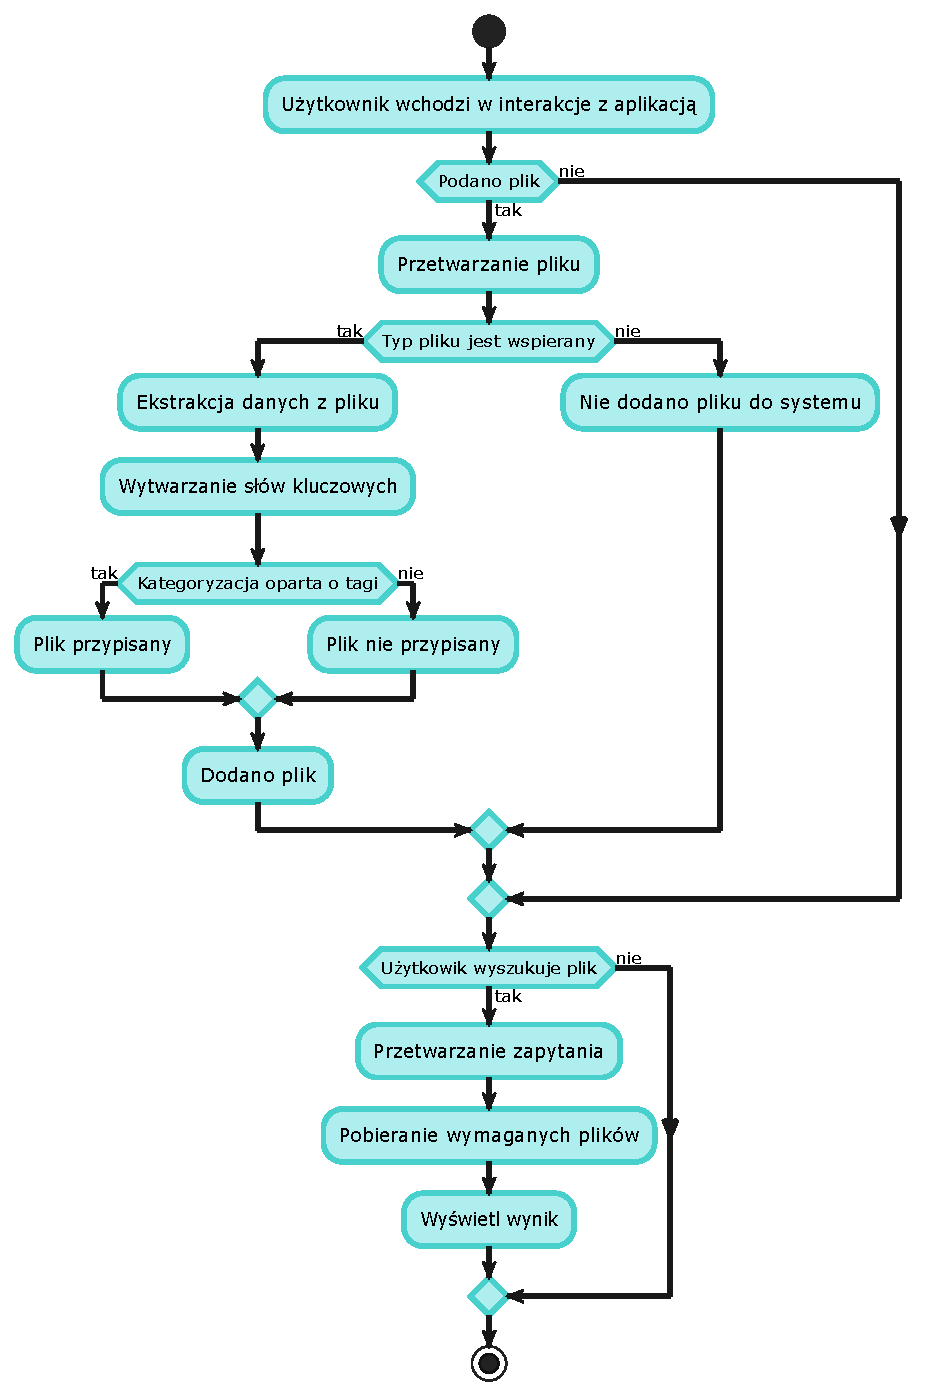
\includegraphics[width=0.8\textwidth]{img/plantuml.pdf}
\caption{Diagram aktywności końcowej aplikacji.}
\end{figure}
\newpage
\clearpage
\subsection{Ograniczenia implementacji}
\subsubsection*{Organizacja plików}
Podczas tworzenia systemu napotkano problem dotyczący modułu organizacji danych, a dokładniej automatycznego tworzenia struktur katalogów. Proces ten wymaga wzięcia pod uwagę wielu warunków co sprawia, że koszty implementacji są niewspółmierne do oczekiwanych wyników. Przykładowe wymagania zostały wypisanie poniżej.
\begin{enumerate}
	\item Występowanie niejednoznacznych lub nakładających się słów kluczowych\break w treści pliku może prowadzić do niepewności w kategoryzacji. Jeśli słowo kluczowe jest powiązane z wieloma kategoriami lub jeśli różne pliki zawierają podobne słowa kluczowe o różnych znaczeniach kontekstowych, może to spowodować błędną klasyfikację plików do nieprawidłowych katalogów.
	\item Zmienność w użyciu słów kluczowych, takich jak synonimy, skróty lub różnice w pisowni, może stanowić wyzwanie w dokładnej identyfikacji i wyodrębnianiu odpowiednich słów kluczowych z zawartości pliku. 
\end{enumerate}
Zważając na ograniczenia czasowe, została podjęta decyzja o ograniczeniu modułu organizacji danych do implementacji systemu generacji słów kluczowych z zawartości plików oraz łączenia plików ze względu na nie. Schemat działania asocjacji plików został przedstawiony w rozdziale 2.3.
\subsubsection*{Implementacja abstrakcyjnego tworzenia streszczeń}
Abstrakcyjna generacja streszczeń jest procesem wymagającym posiadania zestawu treningowego złożonych z streszczeń i przypisanym im tekstów początkowych. Jest to proces czasochłonny, lecz jakościowo przewyższa streszczenia metodami ekstraktywnymi. \par
Samodzielna kreacja takiego systemu nie jest optymalna pod względem ilości zasobów potrzebnych do uczenia modelu oraz zasobów pamięciowych przeznaczonych na działanie całej aplikacji. Istnieje jednak rozwiązanie tego problemu\break z pomocą dostępnych na rynku \textit{API}. Wiele narzędzi zostało wytrenowane na ogromnych zestawach danych w celu tworzenia takich abstraktów, tak jak oferowany przez \textit{OpenAI} system streszczeń oparty na \textit{GPT-3}.
\subsection{Obsługiwane rodzaje plików}
%% ########################################################
System w aktualnym stanie realizacji jest przystosowany do obsługi plików w formatach, między innymi takich jak \textit{PDF} oraz \textit{CSV}. W zależności od struktury pliku, system udostępnia stosowne funkcjonalności, co jest opisane poniżej. Do plików przypisujemy etykietę opisującą rodzaj pliku, lecz jest ona odrębną jednostką od słów kluczowych generowanych na podstawie zawartości pliku.
\subsubsection*{Pliki PDF}
Proces obsługi plików PDF jest zależny od wielu czynników. Najprostszymi plikami do analizy są artykuły posiadające zakładki (\textit{ang. outlines}) o ujednoliconej strukturze, zawierające jedynie tekst. Słowo \textit{outlines} jest zwrotem specyficznym dla plików PDF i są potrzebne do ustalenia tytułu danego pliku. Wynika to z faktu, że rzadko nazwa pliku koresponduje tytułowi zawartości.\par
System wykorzystuje potokowanie zawartości w celu ekstrakcji tekstu, obrazów oraz tabel. Oznacza to, że aplikacja nie ``widzi'' dokumentu, lecz pobiera informacje z kodu źródłowego pliku. Działanie aplikacji jest oparte o sam tekst.\break Na potrzeby aplikacji, takie fragmenty jak tabele czy grafiki są jedynie przeszkodą, ponieważ nie powinny one wpływać na wynik algorytmu streszczania. Część elementów tabelarycznych jest niepoprawnie podpisywana jako tekst, co może przyczynić się do generacji niezrozumiałych streszczeń. 
\subsubsection*{Pliki tabelaryczne}
Podstawowym zachowaniem aplikacji w obliczu plików zawierających dane tabelaryczne jest generacja opisu zgodnie z następującymi krokami. Dla każdej kolumny pobierana jest jej nazwa oraz rodzaj danych zawartych w niej. Ze względu na specyfikę pliku, generacja słów kluczy może przebiec na dwa sposoby: etykietami zostają nazwy kolumn lub użytkownik samodzielnie je dodaje.\par
Żadne z wymienionych podejść, nie jest wystarczające. Nazewnictwo kolumn tworzonych tabel nie jest ustandaryzowane, ani wymagane, co może powodować wytworzenie mylących lub bezużytecznych nagłówków. Dlatego w pełni zautomatyzowany algorytm może działać wadliwie. Drugie podejście wymaga od użytkownika większego wkładu w ten proces. Poprawne etykietowanie wprowadzanego pliku, wymaga wiedzy dotyczącej zawartości zestawu danych i informacji o pliku. Z wymienionych powodów, w implementacji są stosowane oba sposoby.
%\subsection{Przykłady implementacji}
%Poniższy dział zaprezentuje przykładowe implementacje wyżej wymienionych funkcjonalności.
%\begin{enumerate}
%	\item wyszukiwanie
%	\begin{figure}[h!]
%		\centering
% 		\includegraphics[width=\textwidth]{img/file\_search\_code.jpg}
%  		\caption{Implementacja wyszukiwania pliku}
%	\end{figure}
%\end{enumerate}
\subsection{Możliwości rozwoju i wykorzystania aplikacji}
Wspomniane funkcjonalności to jedynie początek istnienia tego systemu. Stworzenie dodatkowych zdolności programu jest uproszczone dzięki oparciu systemu\break o odpowiedzi w postaci komunikatu HTTP, zamiast stosowania szablonów, jak to jest zwykle przy standardowym projektowaniu z użyciem Python Flask. Baza danych wykorzystana w projekcie, MongoDB, jest bazą typu NoSQL, która umożliwia przechowywanie informacji w nieustrukturyzowany sposób. Dzięki czemu tabele można wypełnić dowolnymi wartościami, a sama aplikacja wyświetla wyszystkie elementy tabeli dla wyszukiwanego obiektu.\par
\subsubsection{Ekspansja działań dotyczących danych tabelarycznych}
Aktualny system pozwala na implementacje metod wstępnego przetwarzania danych (\textit{ang. preprocessing}) z wnętrza aplikacji. Preprocessing oznacza zbiór działań mających na celu obróbkę i przygotowanie danych do dalszej manipulacji. Do takich działań należą usunięcie wartości brakujących, filtracja czy usuniecie wartości odstajacych. \par
Celem stworzenia systemu jest automatyzacja procesów związanych z przechowywaniem informacji. Dodanie takich możliwości jak łączenie tabel w pojedyńcze pliki czy, w przypadku plików zawierających kilka osobnych arkuszy danych, pozwolenie na rozdzielenie ich na osobne pliki, powinno być celem kolejnych implementacji.
\subsubsection{Identyfikacja obrazów}
Identyfikacja obrazów może przysłużyć się sukcesowi systemu. Dla człowieka proces identyfikacji elementów obrazu dzieje się podświadomie, a w przypadku programu, jest on w stanie rozpoznać i przypisać grafikę do odpowiedniej kategorii, jedynie\break w sytuacji gdy jest on zaprogramowany do wykrywania ich. Komputery kategoryzują obrazy, porównując układ pikseli wejściowego obrazu ze schematami zapisanymi\break w systemie. Z punktu widzenia maszyny, obraz jest ustrukturyzowaną macierzą liczb, której każdy element zawiera informacje o nasyceniu i kolorze piksela. Aby stworzyć system odpowiedzialny za kategoryzację obrazów, należy przejść przez następujące kroki:
\begin{enumerate}
	\item gromadzenie danych,
	\item przygotowanie danych,
	\item wybór, trenowanie i testowanie modelu,
	\item wprowadzenie modelu do systemu.
\end{enumerate}
Najważniejszym elementem skutecznego systemu rozpoznawania obrazów jest dobrze skonstruowany zbiór danych. Etap gromadzenia danych obejmuje pozyskiwanie różnorodnych obrazów reprezentujących obiekty, sceny lub wzorce, które system nauczy się rozpoznawać. Kompleksowy zbiór danych przyczynia się do zdolności systemu do uogólniania swojego zrozumienia w różnych scenariuszach.\par
Przygotowanie danych (\textit{ang. Preprocessing}) to proces przekształcania i udoskonalania zebranych danych, aby były odpowiednie do przeprowadzenia treningu systemu. Może to obejmować takie zadania, jak usuwanie niespójności, zmiana rozmiaru obrazów do spójnego formatu i normalizacja wartości pikseli. Skuteczny preprocessing danych wspomaga zdolność modelu do nauki istotnych wzorców z danych.\par
Kluczową decyzją jest wybór architektury modelu, która powinna być dostosowana do wymagań zadania i zasobów obliczeniowych. Określa ona sposób, w jaki system będzie przetwarzał i interpretował dane wejściowe. Trening modelu to proces uczenia wybranej architektury rozpoznawania wzorców i cech w danych treningowych. Osiąga się to poprzez iteracyjną optymalizację, w której parametry modelu są dostosowywane w celu zminimalizowania różnicy między przewidywanymi a rzeczywistymi wynikami. Trening trwa do momentu, aż model osiągnie optymalny poziom dokładności i uogólnienia, który sprawi, że będzie on biegły\ w rozpoznawaniu obiektów na obrazach. \par
Ostatnim etapem, poprzedzającym implementacje modelu, jest testowanie wytrenowanego modelu. Jest ono niezbędne do oceny jego wydajności dla nowych danych. System jest zasilany obrazami, których nie napotkał podczas szkolenia, umożliwiając ocenę jego zdolności do generalizacji. Metryki takie jak dokładność, precyzja i czułość zapewniają wgląd w mocne i słabe strony modelu. Rygorystyczne testowanie pomaga w dostrojeniu modelu w celu uzyskania lepszej wydajności \cite{imagg}.\par
Powszechnie dostępne, ogromne bazy danych, takie jak \textit{Pascal VOC} czy \textit{ImageNet}, pozwalają na stworzenie i wdrożenie takiego modelu. Zawierają one mnóstwo oznaczonych wzorców opisujących obiekty znajdujące sie na obrazach. 
%% ########################################################
\newpage
\section*{Podsumowanie}
\addcontentsline{toc}{section}{Podsumowanie}
W ramach pracy zaprezentowano projekt aplikacji, która umożliwiłaby komfortowe przechowywanie danych oraz zmniejszenie ingerencji użytkownika w proces interpretacji plików. Opisano funkcjonalności aplikacji oraz możliwe rozszerzenia aplikacji\break w dalszym ciągu rozwoju. \par
Jednym z intrygujących wyzwań była implementacja ekstrakcji tekstu z plików PDF. Analiza tego procesu skupiła się głównie na wyodrębnianiu tekstu bezpośrednio ze strumienia pliku, podkreślając złożoność i interpretowania struktur dokumentów. Skłoniło to również do rozważenia alternatywnych metod ekstrakcji, takich jak optyczne rozpoznawanie znaków (OCR). \par
Ponadto, chociaż aplikacja oferuje możliwość wyszukiwania, ważne jest, aby uznać jej potencjalne ograniczenia, szczególnie w przypadkach, gdy błędy ekstrakcji tekstu sprawiają, że słowa kluczowe są nieskuteczne dla dokładnych wyników wyszukiwania.\par
Architektura aplikacji pozwala jednak na jej przyszłą rozbudowę i ulepszenie. Integracja z zewnętrznymi interfejsami API lub dodanie rozszerzeń możę zwiększyć jej funkcjonalność. Co więcej, wykorzystanie bazy danych NoSQL zapewnia elastyczność w przechowywaniu różnych typów informacji, przyczyniając się do skalowalności aplikacji. Niemniej jednak ważne jest, aby zdać sobie sprawę, że wdrożenie kategoryzacji według tematów w celu tworzenia katalogów w aplikacji stanowi znaczące przedsięwzięcie. Osiągnięcie tej funkcjonalności wymaga znacznych inwestycji w czas i zasoby, ponieważ opiera się na płynnym funkcjonowaniu różnych połączonych ze sobą komponentów w ekosystemie aplikacji.
%% ########################################################
\newpage
\listoffigures
\addcontentsline{toc}{section}{Spis Rysunków}
\newpage
\addcontentsline{toc}{section}{Bibliografia}
\bibliographystyle{IEEEtran}
\bibliography{biblioteka}
\end{document}